% Part 4 guided reading session. Build from this directory with make.
\documentclass[11pt]{article}
\newcommand{\iliadpart}{4. Identifying belief geometry in transformers}
\newcommand{\iliadhandout}{Reading guide}
\usepackage{iliad-reading-guide}
\graphicspath{{../slides/figures/}}

\hypersetup{
  pdftitle={Computational Mechanics: Identifying belief geometry in transformers},
  pdfauthor={Xavier Poncini}
}

\begin{document}
\makeiliadreadingtitle

So far, we have developed the conceptual framework of computational mechanics.
We now ask whether neural networks trained for next-token prediction---including
transformers and recurrent architectures---learn the predictive structures
identified by that framework. You will read selected sections of two papers,
then discuss their evidence and limitations in small groups.

\begin{sessionplan}
  \begin{enumerate}[nosep]
    \item \textbf{Readings (75 minutes).} Begin with the main reading and use
      the route below. Continue to the extension if time permits.
    \item \textbf{Discussion (30 minutes).} Form groups of three or four.
      Compare what you found convincing, confusing, or incomplete; use the
      prompts on page 2 if useful.
  \end{enumerate}
\end{sessionplan}

\guideheading{Readings}
Prioritise the main reading. If you can answer its evaluation question, you
have probably understood one of its central results. If time is short, skim
the extension overview before deciding whether to continue.

\begin{reading}[Main]
  {Transformers represent belief state geometry in their residual stream}
  {https://arxiv.org/pdf/2405.15943}
  \begin{readingroute}
    \routeitem{Skim}{Sections 1, 2.1, and 2.2.}
    \routeitem{Read}{Sections 2.3 and 3--5.}
    \routeitem{Evaluation}{Explain Figure 6D. What do the comparison and
      shuffle control establish?}
  \end{readingroute}

  \readingoverview{This paper presents evidence that transformers trained on
  HMM-generated sequences encode belief-state geometry in their residual
  streams. The claim is tested on the Mess3 and Random--Random--XOR (RRXOR)
  processes. For each process, the authors fit an affine map from residual
  activations to the exact HMM belief state and evaluate it using mean-squared
  error (MSE). The error decreases over training checkpoints. A shuffle
  control tests whether low MSE could arise merely because a high-dimensional
  activation space is being projected into a low-dimensional belief space.}
\end{reading}

\newpage
\begin{reading}[Extension]
  {Neural networks leverage nominally quantum and post-quantum representations}
  {https://arxiv.org/pdf/2507.07432}
  \begin{readingroute}
    \routeitem{Skim}{Sections 1--3.}
    \routeitem{Read}{Sections 4--8.}
    \routeitem{Evaluation}{Explain Figure 3B. How are the light-blue and light-orange
      plots related to the corresponding dark-blue and dark-orange plots?}
  \end{readingroute}

  \readingoverview{This paper extends the question from HMMs to generalised
  hidden Markov models (GHMMs). As in Part 3, a GHMM retains the matrix-product
  expression for output probabilities while relaxing the entrywise
  probabilistic constraints on its internal matrices. This larger model class
  can realise some processes in finite dimension even when a corresponding
  minimal HMM requires exponentially many more hidden states.

  Using techniques related to those in the main reading, the authors study
  transformers, LSTMs, RNNs, and GRUs trained on processes with distinct GHMM
  and HMM realisations. Their results indicate that the networks learn
  belief-state representations associated with the lower-dimensional GHMM
  realisation. The finding suggests that neural networks can select among
  representational model classes in ways that capture dimensionality savings.}
\end{reading}

\guideheading{Discussion}
Here are some prompts to consider:
\begin{itemize}
  \item What is the most convincing evidence that transformers represent
    belief-state geometry? What is the least convincing?
  \item What additional experiment would most strengthen or weaken the claim?
  \item Which alternative hypotheses could explain the reported results?
  \item Can you explain each element of the diagram below---including the
    generative HMM, Bayesian updating, transformer activations, fitted affine
    map, and belief-state geometry?
\end{itemize}

\begin{center}
  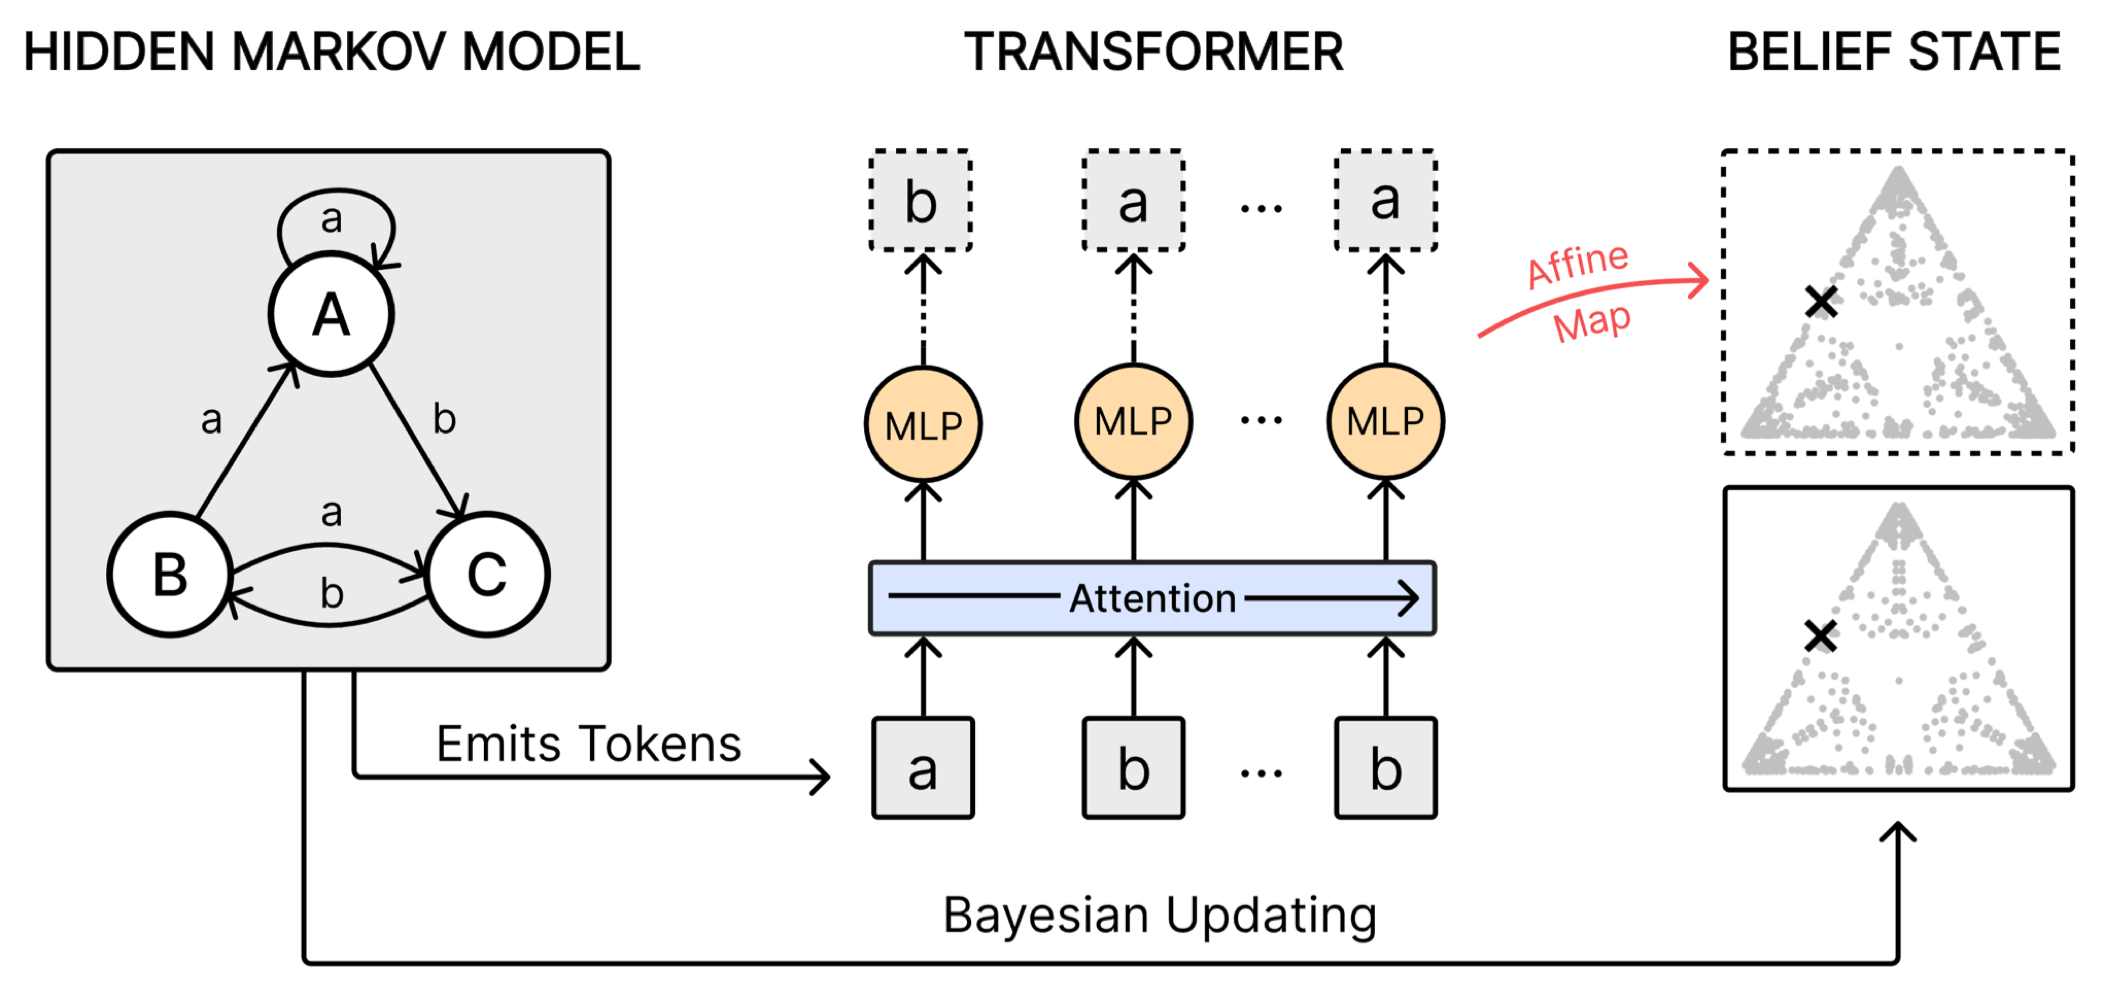
\includegraphics[width=0.88\linewidth,height=49mm,keepaspectratio]
    {shai-belief-state-geometry}
\end{center}

\end{document}
